\documentclass[11pt,a4paper]{article}

% --- Packages ---
\usepackage[utf8]{inputenc} 
\usepackage[T1]{fontenc}    
\usepackage{geometry}       
\geometry{
    a4paper,
    total={170mm,257mm},
    left=25mm,
    top=25mm,
}
\usepackage{graphicx}       
\usepackage{amsmath, amssymb} 
\usepackage{hyperref}       
\hypersetup{                
    colorlinks=true,
    linkcolor=blue,
    urlcolor=cyan,
}
\usepackage{indentfirst}
\usepackage{float}
\usepackage{listings}
\usepackage{xcolor}
\usepackage{tikz}
\usetikzlibrary{arrows.meta, positioning, shapes.geometric}

\lstset{
    basicstyle=\ttfamily\footnotesize,
    commentstyle=\color{green!60!black},
    keywordstyle=\color{blue},
    numbers=left,
    numberstyle=\tiny\color{gray},
    frame=single,
}

% Title and labeling
\title{Sampling and Reconstruction \\ [1ex] \large ECSE 313 Group 16 Lab 4 Report}
\author{Nathaniel Hahn and Donovan Crowley}
\date{\today}

% Body
\begin{document}

\maketitle 

\tableofcontents 
\newpage

\section{Sampling and Reconstruction Using Sample-and-Hold}

\begin{figure}[H]
    \centering
    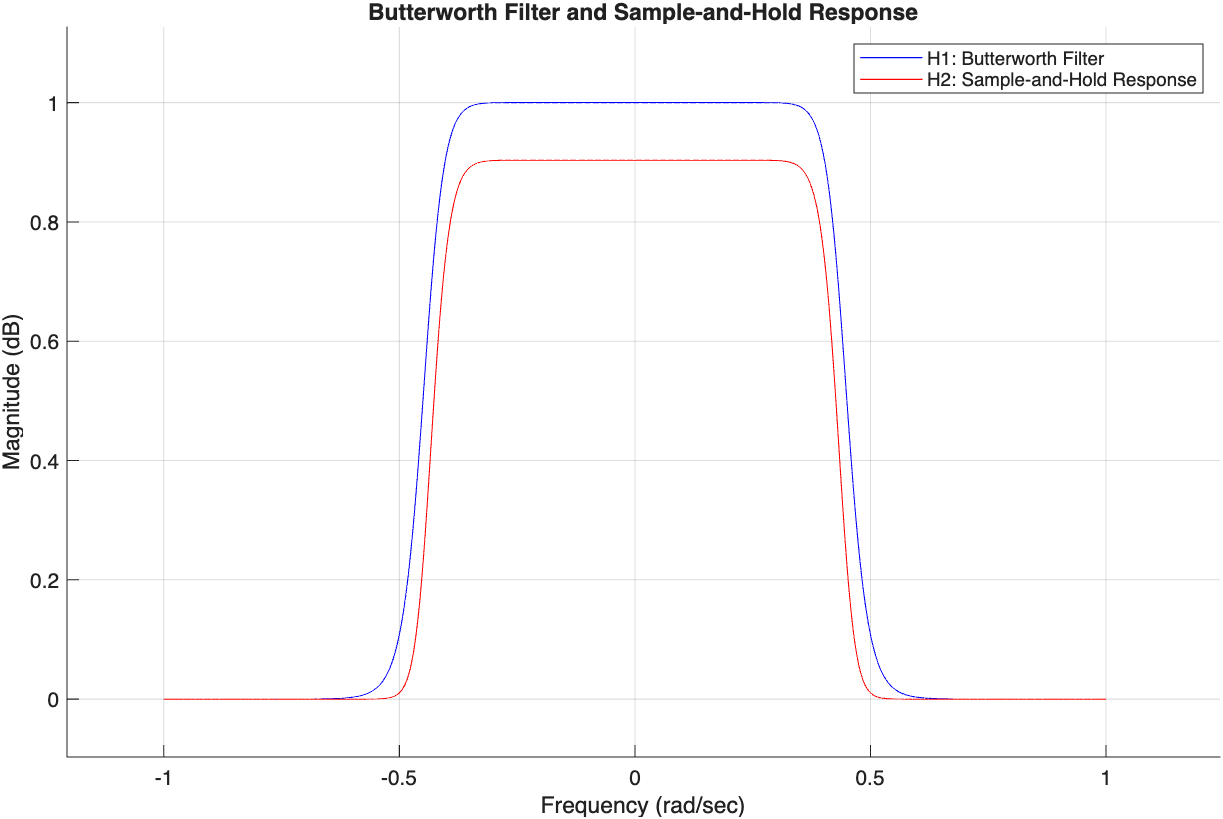
\includegraphics[width=0.8\textwidth]{../Figure_1.png}
    \caption{Magnitude Response of Butterworth Filter and Sample-and-Hold Response}
\end{figure}
The magnitude of the Butterforth filter is greater than that with the sample-and-hold device. 
The magnitude response of the sample-and-hold acts as a low pass filter. For high quality audio CD players, a low pass filter smooths the signal and improves audio clarity.

\section{Sampling and Reconstruction Using An Impulse Generator}

\begin{figure}[H]
    \centering
    
\includegraphics[width=0.4\textwidth]{../image2.png}
    \caption{Input/Output Signals at 0.3 Sec Pulse}
\end{figure}

The aliasing in Figure 2 is represented by the yellow curve.

\begin{figure}[H]
    \centering
    
\includegraphics[width=0.4\textwidth]{../image3.png}
    \caption{Output Signal and Frequency Spectrum at 0.3 Sec Pulse}
\end{figure}

\begin{figure}[H]
    \centering
    
\includegraphics[width=0.4\textwidth]{../image4.png}
    \caption{Input/Output Signals at 0.1 Sec Pulse}
\end{figure}

\begin{figure}[H]
    \centering
    
\includegraphics[width=0.4\textwidth]{../image5.png}
    \caption{Output Signal and Frequency Spectrum at 0.1 Sec Pulse}
\end{figure}

The aliasing curves in Figure 4 have a smaller width than those in Figure 2. 
Additionally, the spectral density in Figure 5 has a lower magnitude intensity than that in Figure 3.

% ADD MORE HERE !!

\begin{figure}[H]
    \centering
    
\includegraphics[width=0.4\textwidth]{../image7.png}
    \caption{Input/Output Signals at 0.1 Sec Pulse}
\end{figure}

\begin{figure}[H]
    \centering
    
\includegraphics[width=0.4\textwidth]{../image6.png}
    \caption{Output Signal and Frequency Spectrum at 0.3 Sec Pulse with 0.8 Hz}
\end{figure}

\begin{figure}[H]
    \centering
    
\includegraphics[width=0.4\textwidth]{../image8.png}
    \caption{Input/Output Signals with Butterworth Filter}
\end{figure}

\begin{figure}[H]
    \centering
    
\includegraphics[width=0.4\textwidth]{../image9.png}
    \caption{Output Signal and Frequency Spectrum with Butterworth Filter}
\end{figure}

\section{Sampling and Reconstruction with Sample and Hold}

\begin{figure}[H]
    \centering
    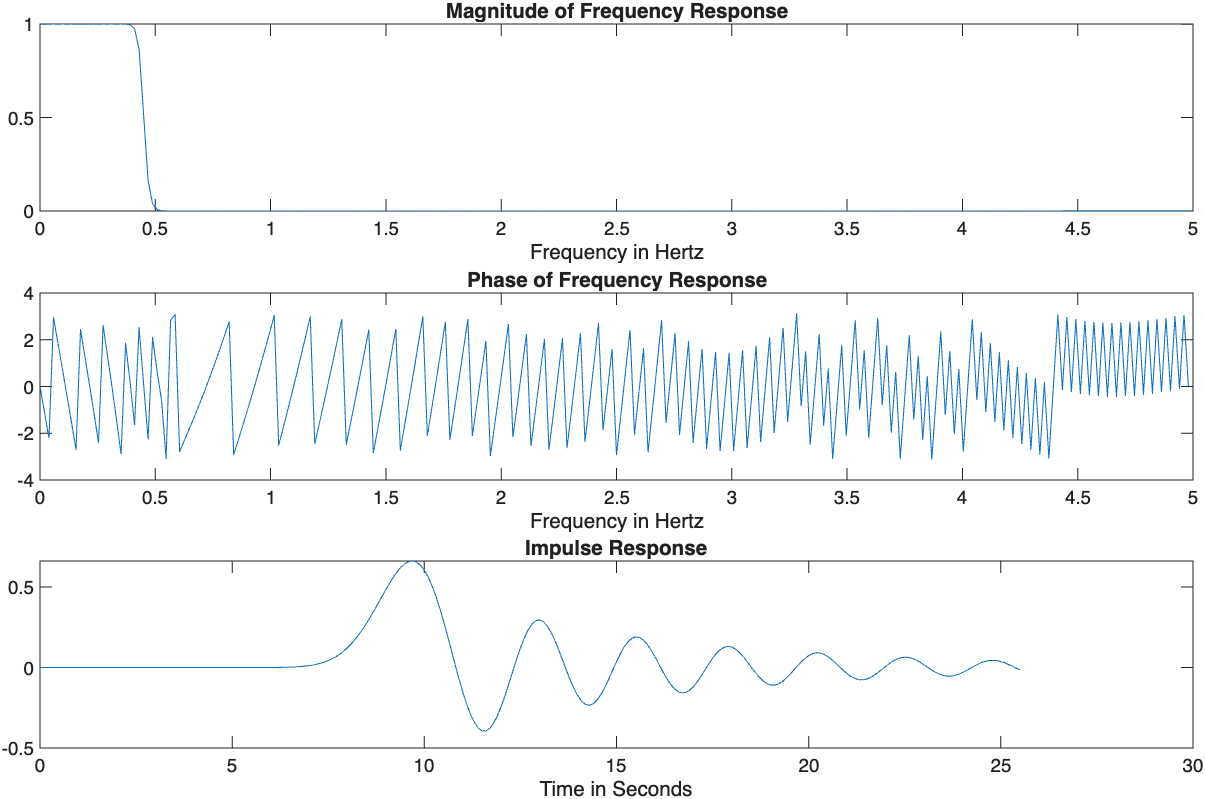
\includegraphics[width=0.4\textwidth]{../56image.png}
    \caption{Sample-and-Hold With Two Scopes}
\end{figure}

\begin{figure}[H]
    \centering
    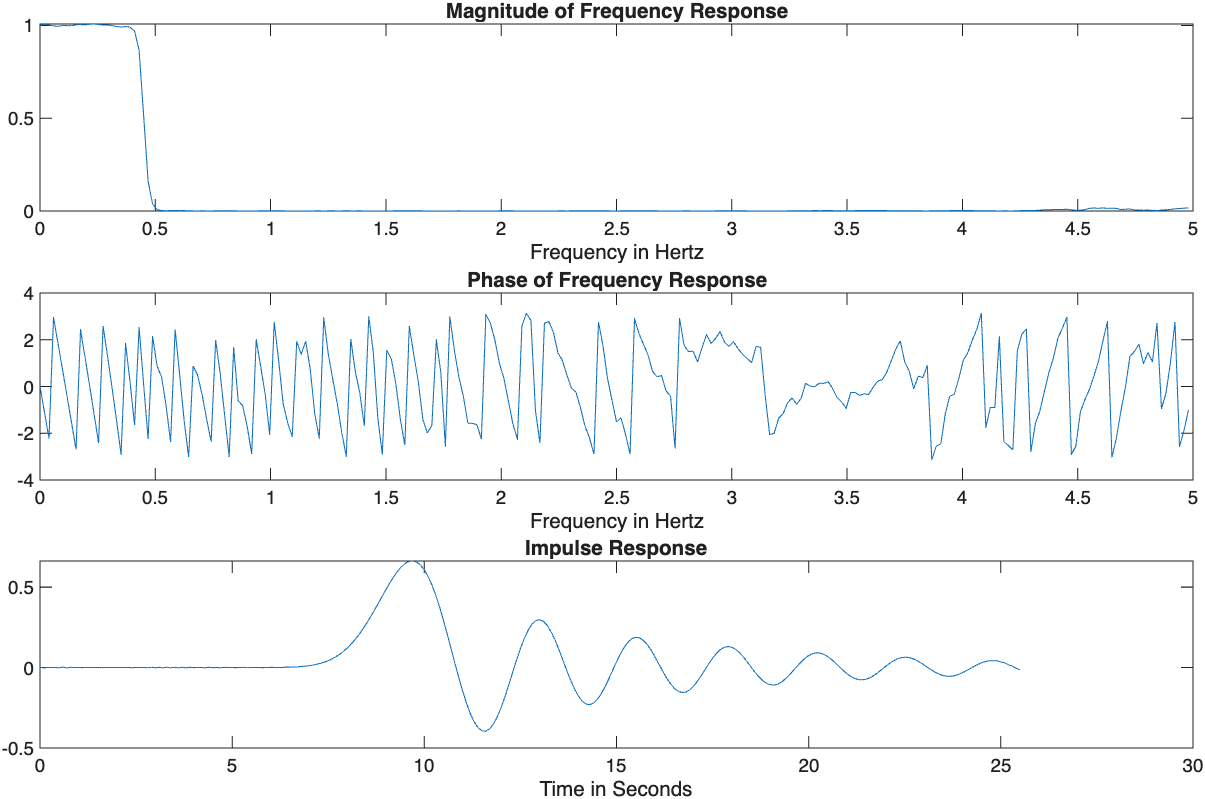
\includegraphics[width=0.4\textwidth]{../56image2.png}
    \caption{Sample-and-Hold With Two Scopes}
\end{figure}

% Add explanation here

\section{Discrete-Time Interpolation}

\begin{figure}[H]
    \centering
    
\includegraphics[width=0.4\textwidth]{../image10.png}
    \caption{Discrete Time Interpolator Scope}
\end{figure}

\begin{figure}[H]
    \centering
    
\includegraphics[width=0.4\textwidth]{../image11.png}
    \caption{Signal.c and Frequency Spectrum}
\end{figure}

\begin{figure}[H]
    \centering
    
\includegraphics[width=0.4\textwidth]{../image12.png}
    \caption{Discrete Time Interpolator Scope With 4 Hz}
\end{figure}

\begin{figure}[H]
    \centering
    
\includegraphics[width=0.4\textwidth]{../image13.png}
    \caption{Signal.c and Frequency Spectrum With 4 Hz}
\end{figure}


\section{Discrete-Time Decimation}



\end{document}
